% Standalone TikZ figure for IEEE paper -- 4-zone architecture (v8)
% Larger ESP32-C6 / OTBR / TB Edge / HaLow radio boxes with extra surrounding
% gap. Total figure: 40 cm x 13 cm.
\documentclass[border=12pt,tikz]{standalone}
\usepackage[T1]{fontenc}
\usepackage{amssymb}
\usepackage{tikz}
\usetikzlibrary{calc,arrows.meta,positioning,fit,backgrounds,decorations.pathmorphing}
\begin{document}
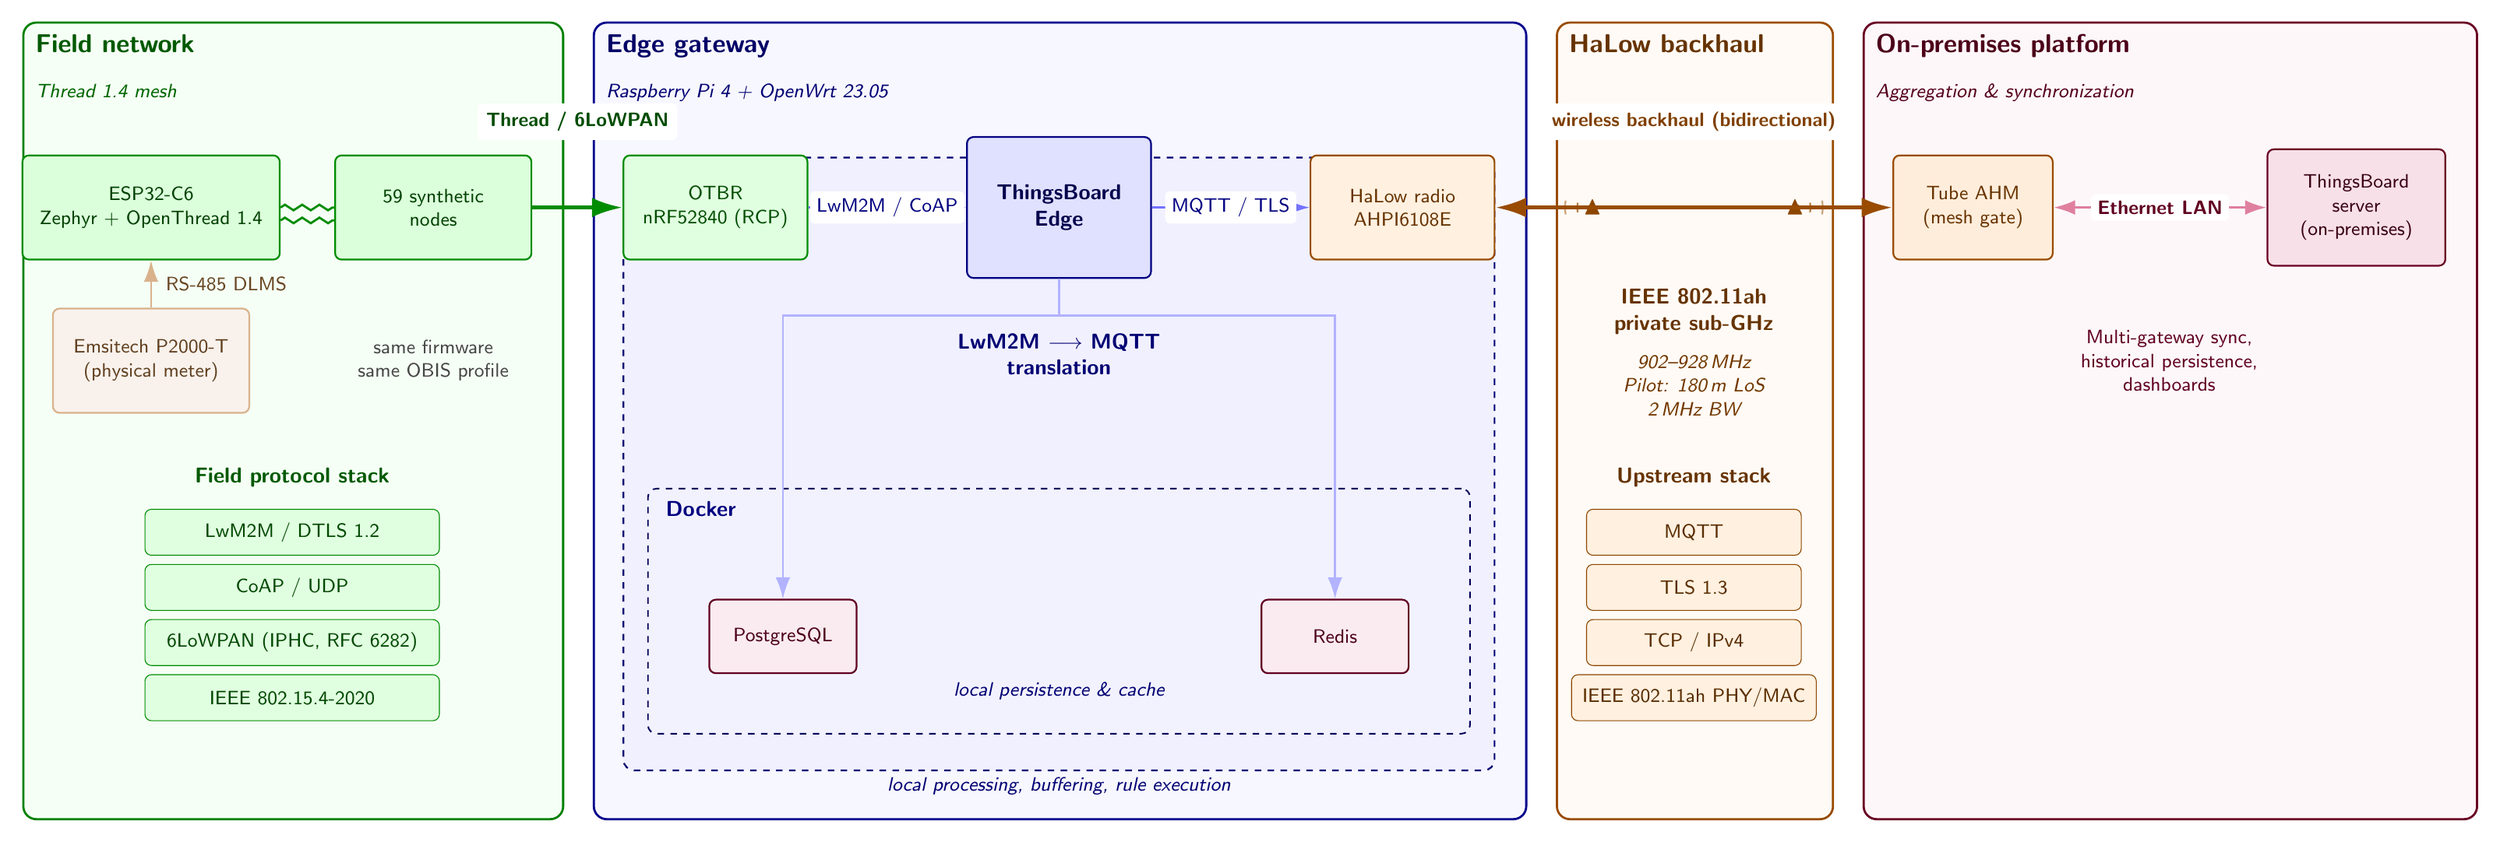
\begin{tikzpicture}[
  font=\sffamily\small,
  % --- zone backgrounds ---
  Z1/.style={rounded corners=6pt, draw=green!50!black,  fill=green!4,  line width=1pt},
  Z2/.style={rounded corners=6pt, draw=blue!55!black,   fill=blue!3,   line width=1pt},
  Z3/.style={rounded corners=6pt, draw=orange!60!black, fill=orange!4, line width=1pt},
  Z4/.style={rounded corners=6pt, draw=purple!55!black, fill=purple!3, line width=1pt},
  zlab/.style={font=\sffamily\bfseries\large, inner sep=6pt},
  zsub/.style={font=\sffamily\small\itshape, inner sep=6pt},
  % --- components ---
  comp/.style={rounded corners=3pt, draw, line width=0.8pt, inner sep=8pt,
               minimum height=1.4cm, align=center,
               font=\sffamily\small, fill=white},
  % Big nodes/devices (user-requested extra space):
  node1/.style ={comp, draw=green!55!black,  fill=green!14, minimum width=3.2cm, minimum height=1.7cm, text=green!25!black},
  meter/.style ={comp, draw=brown!60,        fill=brown!10, minimum width=3.2cm, minimum height=1.7cm, text=brown!50!black},
  otbr/.style  ={comp, draw=green!55!black,  fill=green!12, minimum width=3.0cm, minimum height=1.7cm, text=green!30!black},
  halow/.style ={comp, draw=orange!60!black, fill=orange!12,minimum width=3.0cm, minimum height=1.7cm, text=orange!40!black},
  tbedge/.style={comp, draw=blue!50!black,   fill=blue!12,  minimum width=3.0cm, minimum height=2.3cm, text=blue!30!black, font=\sffamily\normalsize\bfseries},
  % Other devices (kept proportional):
  dbedge/.style={comp, draw=purple!50!black, fill=purple!8, minimum width=2.4cm, minimum height=1.2cm, text=purple!40!black, font=\sffamily\small},
  meshgt/.style={comp, draw=orange!60!black, fill=orange!14,minimum width=2.6cm, minimum height=1.7cm, text=orange!40!black},
  server/.style={comp, draw=purple!55!black, fill=purple!12,minimum width=2.9cm, minimum height=1.9cm, text=purple!30!black},
  gwbox/.style ={rounded corners=5pt, draw=blue!45!black, fill=blue!6,  line width=0.8pt, dashed},
  dockbox/.style={rounded corners=4pt, draw=blue!35!black, fill=blue!5, line width=0.7pt, dashed},
  % --- arrows ---
  arr/.style       ={-{Latex[length=3.5mm,width=2.4mm]}, line width=1pt},
  arrthick/.style  ={-{Latex[length=5mm,width=3.2mm]}, line width=2pt},
  arrbidir/.style  ={{Latex[length=5mm,width=3.2mm]}-{Latex[length=5mm,width=3.2mm]}, line width=2pt},
  arrbidirfin/.style={{Latex[length=3.5mm,width=2.4mm]}-{Latex[length=3.5mm,width=2.4mm]}, line width=1.2pt},
  % --- protocol chips ---
  protoG/.style={rounded corners=3pt, draw=green!55!black, fill=green!12,
                 font=\sffamily\small, inner sep=5pt, minimum height=0.75cm,
                 text=green!28!black, minimum width=4.8cm, align=center},
  protoO/.style={rounded corners=3pt, draw=orange!55!black, fill=orange!12,
                 font=\sffamily\small, inner sep=5pt, minimum height=0.75cm,
                 text=orange!35!black, minimum width=3.5cm, align=center},
  % --- mesh decoration ---
  meshlink/.style={green!55!black, line width=1pt, decorate,
                   decoration={zigzag, amplitude=1.3pt, segment length=8pt}},
  % --- floating cross-zone label ---
  xzlabel/.style={font=\sffamily\small\bfseries, fill=white, inner sep=4pt, rounded corners=2pt},
]

% =================================================================
%  ZONE 1 --- Field network (x: 0 to 8.8, width 8.8)
%  Inner 0.5 to 8.3 (7.8). 2 nodes 3.2 + 1 gap 1.4 = 7.8
% =================================================================
\node[Z1, minimum width=8.8cm, minimum height=13cm,
      anchor=south west] (Z1F) at (0,0) {};
\node[zlab, green!35!black, anchor=north west]
  at (Z1F.north west) {Field network};
\node[zsub, green!40!black, anchor=north west]
  at ($(Z1F.north west)+(0,-0.8)$) {Thread 1.4 mesh};

% Nodes: NP at 2.1, NS at 6.7 (centers, with 1.4 gap)
\node[node1] (NP) at (2.1, 10.0) {ESP32-C6\\Zephyr + OpenThread 1.4};
\node[meter] (MP) at (2.1, 7.5)  {Emsitech P2000-T\\(physical meter)};
\draw[arr, brown!60] (MP.north) -- (NP.south)
  node[midway, right=3pt, font=\sffamily\small, brown!55!black]
  {RS-485 DLMS};

\node[node1] (NS) at (6.7, 10.0) {59 synthetic\\nodes};
\node[font=\sffamily\small, gray!55!black, align=center]
  at (6.7, 7.5) {same firmware\\same OBIS profile};

% Thread mesh links between the two node groups
\draw[meshlink] (NP.east) -- (NS.west);
\draw[meshlink] ([yshift=-6pt]NP.east) -- ([yshift=-6pt]NS.west);

% Field protocol stack (centered in zone)
\node[font=\sffamily\normalsize\bfseries, green!35!black]
  at (4.4, 5.6) {Field protocol stack};
\node[protoG] at (4.4, 4.7) {LwM2M / DTLS 1.2};
\node[protoG] at (4.4, 3.8) {CoAP / UDP};
\node[protoG] at (4.4, 2.9) {6LoWPAN (IPHC, RFC 6282)};
\node[protoG] at (4.4, 2.0) {IEEE 802.15.4-2020};

% =================================================================
%  ZONE 2 --- Edge gateway (x: 9.3 to 24.5, width 15.2)
%  Inner 9.8 to 24.0 (14.2). 3 boxes 3.0 + 2 gaps 2.6 = 14.2
% =================================================================
\node[Z2, minimum width=15.2cm, minimum height=13cm,
      anchor=south west] (Z2F) at (9.3,0) {};
\node[zlab, blue!40!black, anchor=north west]
  at (Z2F.north west) {Edge gateway};
\node[zsub, blue!45!black, anchor=north west]
  at ($(Z2F.north west)+(0,-0.8)$) {Raspberry Pi 4 + OpenWrt 23.05};

% Inner gateway dashed box
\node[gwbox, minimum width=14.2cm, minimum height=10cm,
      anchor=south] (GW) at (16.9, 0.8) {};

% Top row: OTBR (11.3) | TBE (16.9) | HAL (22.5) -- 2.6cm gaps
\node[otbr]  (OTBR) at (11.3, 10.0) {OTBR\\nRF52840 (RCP)};
\node[tbedge](TBE)  at (16.9, 10.0) {ThingsBoard\\Edge};
\node[halow] (HAL)  at (22.5, 10.0) {HaLow radio\\AHPI6108E};

% Translation label below TB Edge
\node[font=\sffamily\normalsize\bfseries\itshape, blue!45!black, align=center]
  at (16.9, 7.6) {LwM2M $\longrightarrow$ MQTT\\translation};

% Internal protocol-flow arrows: labels sit ON the arrow line
\draw[arr, blue!55] (OTBR.east) -- (TBE.west)
  node[midway, font=\sffamily\small, text=blue!50!black,
       fill=white, inner sep=3pt, rounded corners=2pt] {LwM2M / CoAP};
\draw[arr, blue!55] (TBE.east) -- (HAL.west)
  node[midway, font=\sffamily\small, text=blue!50!black,
       fill=white, inner sep=3pt, rounded corners=2pt] {MQTT / TLS};

% Docker box and sidecar databases
\node[dockbox, minimum width=13.4cm, minimum height=4.0cm,
      anchor=south] (DOCK) at (16.9, 1.4) {};
\node[font=\sffamily\normalsize\bfseries\itshape, blue!50!black, anchor=north west]
  at ($(DOCK.north west)+(0.18,-0.1)$) {Docker};

% PG and Redis as sidecars (further apart given wider zone)
\node[dbedge] (PG) at (12.4, 3.0) {PostgreSQL};
\node[dbedge] (RD) at (21.4, 3.0) {Redis};

% TB Edge -> DBs (sidecars)
\draw[arr, blue!30] (TBE.south) -- ++(0,-0.6) -| (PG.north);
\draw[arr, blue!30] (TBE.south) -- ++(0,-0.6) -| (RD.north);

% Annotations
\node[font=\sffamily\small\itshape, blue!45!black, align=center]
  at (16.9, 2.1) {local persistence \& cache};
\node[font=\sffamily\small\itshape, blue!45!black, align=center]
  at (16.9, 0.55) {local processing, buffering, rule execution};

% =================================================================
%  ZONE 3 --- HaLow backhaul (x: 25.0 to 29.5, width 4.5)
% =================================================================
\node[Z3, minimum width=4.5cm, minimum height=13cm,
      anchor=south west] (Z3F) at (25.0,0) {};
\node[zlab, orange!40!black, anchor=north west, align=left]
  at (Z3F.north west) {HaLow backhaul};

% Antennas + radio waves
\node[font=\sffamily\large, orange!55!black] at (25.6, 10.0) {$\blacktriangle$};
\node[font=\sffamily\large, orange!55!black] at (28.9, 10.0) {$\blacktriangle$};
\foreach \r/\op in {0.25/0.9, 0.45/0.7, 0.65/0.5} {
  \draw[orange!60!black, line width=0.8pt, opacity=\op]
    (25.80, 10.0) ++(170:\r) arc[start angle=170, end angle=190, radius=\r];
  \draw[orange!60!black, line width=0.8pt, opacity=\op]
    (28.70, 10.0) ++(-10:\r) arc[start angle=-10, end angle=10, radius=\r];
}

% Link description
\node[font=\sffamily\normalsize\bfseries, orange!40!black, align=center]
  at (27.25, 8.3) {IEEE 802.11ah\\private sub-GHz};
\node[font=\sffamily\small\itshape, orange!45!black, align=center]
  at (27.25, 7.1) {902--928\,MHz\\Pilot: 180\,m LoS\\2\,MHz BW};

% Upstream protocol stack
\node[font=\sffamily\normalsize\bfseries, orange!40!black]
  at (27.25, 5.6) {Upstream stack};
\node[protoO] at (27.25, 4.7) {MQTT};
\node[protoO] at (27.25, 3.8) {TLS 1.3};
\node[protoO] at (27.25, 2.9) {TCP / IPv4};
\node[protoO, font=\sffamily\small] at (27.25, 2.0) {IEEE 802.11ah PHY/MAC};

% =================================================================
%  ZONE 4 --- On-premises platform (x: 30.0 to 40.0, width 10.0)
%  Inner 30.5 to 39.5 (9.0). TUBE 2.6 + gap 3.5 + SRV 2.9 = 9.0
% =================================================================
\node[Z4, minimum width=10.0cm, minimum height=13cm,
      anchor=south west] (Z4F) at (30.0,0) {};
\node[zlab, purple!40!black, anchor=north west]
  at (Z4F.north west) {On-premises platform};
\node[zsub, purple!45!black, anchor=north west]
  at ($(Z4F.north west)+(0,-0.8)$) {Aggregation \& synchronization};

% TUBE center 31.8, SRV center 38.05 (3.5 cm gap)
\node[meshgt] (TUBE) at (31.8, 10.0) {Tube AHM\\(mesh gate)};
\node[server] (SRV)  at (38.05, 10.0) {ThingsBoard\\server\\(on-premises)};

% Ethernet LAN (bidirectional, label on the line)
\draw[arrbidirfin, purple!50] (TUBE.east) -- (SRV.west)
  node[midway, font=\sffamily\small\bfseries, text=purple!50!black,
       fill=white, inner sep=3pt, rounded corners=2pt] {Ethernet LAN};

% Server role description
\node[font=\sffamily\small, purple!50!black, align=center]
  at (35.0, 7.5) {Multi-gateway sync,\\historical persistence,\\dashboards};

% =================================================================
%  CROSS-ZONE ARROWS
% =================================================================

% Thread mesh -> OTBR. NS.east at x=8.3, OTBR.west at x=9.8; midpoint 9.05.
\draw[arrthick, green!55!black] (NS.east) -- (OTBR.west);
\node[xzlabel, text=green!30!black] at (9.05, 11.4) {Thread / 6LoWPAN};

% HaLow radio -> Tube AHM. HAL.east at x=24.0, TUBE.west at x=30.5; midpoint 27.25.
\draw[arrbidir, orange!60!black] (HAL.east) -- (TUBE.west);
\node[xzlabel, text=orange!50!black] at (27.25, 11.4)
  {wireless backhaul (bidirectional)};

\end{tikzpicture}
\end{document}
